\section{Summary}
This chapter investigated the interpretation of the learned dynamics into a representation usable by localization and navigation systems.
The Dynamic mapping system was integrated on the MiR-100 as a layered costmap which enable integration of user priorities and blueprint maps as well as the learned dynamics.
The translation from the dynamic representation to costs was split in two.
The map for localization only contains obstacle classified as static.
The costmap used for path planning is determined from the probability for occupancy and the dynamics.
This is done by maintaining an updated estimate of the occupancy and predicting the occupancy to come. 
The estimated occupancy probability is updated with new measurements while considering the confidence in it.
For prediction the Markov representation is used to project the estimated occupancy from the time of the last observation to the time of planning.

The classification and projection is incorporated into the Dynamic mapping system in the Cost interpretor section as shown in figure \ref{fig:cost_interpretor_detail}.

\begin{figure}[htbp]
	\centering
	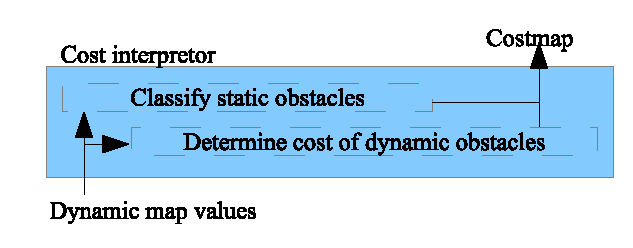
\includegraphics[scale=1]{chapters/cost_interpretation/figures/cost_detail}
	\caption{The Cost interpretor section of the Dynamic mapping system.}
	\label{fig:cost_interpretor_detail}
\end{figure}

